\documentclass[12pt, onecolumn]{IEEEtran}

\usepackage{epsfig,fancybox,verbatim,moreverb}
\usepackage{times}
\usepackage[T1]{fontenc}
%\usepackage{epsfig, graphicx, fancybox, alltt, ifthen, boxit, 
%float, amsmath, amssymb, epsf, array, verbatim, moreverb}


\pagestyle{plain}


\def\inputfig#1{\bgroup\input{#1.tex}\centerline{\box\graph}\egroup}

% Make items flush with left margin
\setlength{\itemindent}{0pt}
\setlength{\leftmargini}{1em}

%\setlength{\oddsidemargin}{0.25in}
%\setlength{\textwidth}{6.0in}
%\setlength{\topmargin}{-0.25in}
%\setlength{\textheight}{8.50in}

\setlength{\oddsidemargin}{0in}
%\setlength{\textwidth}{6.25in}
\setlength{\textwidth}{6.5in}
\setlength{\topmargin}{-0.25in}
%\setlength{\topmargin}{0.25in}
%\setlength{\textheight}{9.25in}
\setlength{\textheight}{8.75in}

%\setlength{\parsep}{5pt}
%\setlength{\parskip}{5pt plus 2pt minus 1pt}
%\def\mnote#1{\marginpar{\tiny {#1}}}
\def\mnote#1{}
\def\note#1{!!~~{\sc #1}} 

%\input{commands}
%\input{/home/agha/agha/ganges/papers/fmoods/lmac}
%\input{/home/agha/agha/ganges/papers/fmoods/mac}
%\input{macros}
%\input{/home/agha/agha/ganges/papers/fmoods/macro}
%\input{/home/agha/agha/ganges/papers/fmoods/commands}

\makeatletter
\def\thebibliography#1{\list
  {[\arabic{enumi}]}{\settowidth\labelwidth{[#1]}\leftmargin\labelwidth
    \advance\leftmargin\labelsep
    \usecounter{enumi}}
    \def\newblock{\hskip .11em plus .33em minus -.07em}
    \sloppy\clubpenalty4000\widowpenalty4000
    \sfcode`\.=1000\relax}

% \newcommand\section{\@startsection {section}{1}{\z@}%
%                                    {-3.5ex \@plus -1ex \@minus -.2ex}%
%                                    {2.3ex \@plus.2ex}%
%                                    {\normalfont\Large\bfseries}}
% \newcommand\subsection{\@startsection{subsection}{2}{\z@}%
%                                      {-3.25ex\@plus -1ex \@minus -.2ex}%
%                                      {1.5ex \@plus .2ex}%
%                                      {\normalfont\large\bfseries}}
% \newcommand\subsubsection{\@startsection{subsubsection}{3}{\z@}%
%                                      {-3.25ex\@plus -1ex \@minus -.2ex}%
%                                      {1.5ex \@plus .2ex}%
%                                      {\normalfont\normalsize\bfseries}}
% \newcommand\paragraph{\@startsection{paragraph}{4}{\z@}%
%                                     {3.25ex \@plus1ex \@minus.2ex}%
%                                     {-1em}%
%                                     {\normalfont\normalsize\bfseries}}
% \newcommand\subparagraph{\@startsection{subparagraph}{5}{\parindent}%
%                                        {3.25ex \@plus1ex \@minus .2ex}%
%                                        {-1em}%
%                                       {\normalfont\normalsize\bfseries}}


\renewcommand\section{\@startsection {section}{1}{\z@}%
                                   {-2.8ex \@plus -1ex \@minus -.2ex}%
                                   {0.85ex \@plus.2ex}%
                                   {\normalfont\Large\bfseries}}
\renewcommand\subsection{\@startsection{subsection}{2}{\z@}%
                                     {-2.8ex\@plus -1ex \@minus -.2ex}%
                                     {0.85ex \@plus .2ex}%
                                     {\normalfont\large\bfseries}}
\renewcommand\subsubsection{\@startsection{subsubsection}{3}{\z@}%
                                     {-2.8ex\@plus -1ex \@minus -.2ex}%
                                     {0.85ex \@plus .2ex}%
                                     {\normalfont\normalsize\bfseries}}
\renewcommand\paragraph{\@startsection{paragraph}{4}{\z@}%
                                    {1.75ex \@plus1ex \@minus.2ex}%
                                    {-1.25em}%
                                    {\normalfont\normalsize\bfseries}}
\renewcommand\subparagraph{\@startsection{subparagraph}{5}{\parindent}%
                                       {2.00ex \@plus1ex \@minus .2ex}%
                                       {-1em}%
                                      {\normalfont\normalsize\bfseries}}
\makeatother

\newcommand{\subsubsubsection}{\paragraph}
\newcommand{\subsubsubsubsection}{\subparagraph}


% Add the compsoc option for Computer Society conferences.
%
% If IEEEtran.cls has not been installed into the LaTeX system files,
% manually specify the path to it like:
% \documentclass[conference]{../sty/IEEEtran}

\usepackage{amsmath}
\usepackage{epsfig}
\usepackage{multirow}


\providecommand{\norm}[1]{\lVert#1\rVert}


% correct bad hyphenation here
\hyphenation{op-tical net-works semi-conduc-tor}


\begin{document}
%
% paper title
% can use linebreaks \\ within to get better formatting as desired

\begin{center}
{\large\bf Quantum Noise Reduction Methods}
\end{center}


\begin{center}
% \begin{minipage}{0.32\linewidth}
%     \begin{center}
%     {\bf Travis Desell}\\
%     \begin{small}
%     Associate Professor\\
%     Department of Software Engineering\\
%     {\it tjdvse@rit.edu}
%     \end{small}
%     \end{center}
% \end{minipage}
% \hfill
\begin{minipage}{0.32\linewidth}
    \begin{center}
    {\bf Steven Szachara}\\
    \begin{small}
    M.S. Data Science\\
    Department of Software Engineering\\
    {\it ss9270@rit.edu}
    %\vspace{\baselineskip}
    \end{small}
    \end{center}
\end{minipage}
\hfill
\begin{minipage}{0.32\linewidth}
    \begin{center}
    {\bf Alexander Jermyn}\\
    \begin{small}
    Student MS Data Science\\
    Department of Something\\
    {\it someone@rit.edu}
    %\vspace{\baselineskip}
    \end{small}
    \end{center}
\end{minipage}
\hfill
\begin{minipage}{0.32\linewidth}
    \begin{center}
    {\bf Daniel Krutz}\\
    \begin{small}
    Professor of Something\\
    Department of Something\\
    {\it someone@rit.edu}
    %\vspace{\baselineskip}
    \end{small}
    \end{center}
\end{minipage}
\end{center}


\IEEEpeerreviewmaketitle
\section{Introduction}
\label{ch:intro}

\section{Background}
\label{ch:background}
% Introduce qiskit package
% \subsection{Quantum Computing and Classical Computing Overview}
\label{sec:quantumoverview}

\cite{feng_quantum_2023}
Quantum state before measurement is a superposition of all possible qubit outputs weighted by their probabilities.

% approach
To contextualize our project, as the subject and topic of quantum computing does have a niche quality, we will take this section to lay the foundation of the quantum vs. classical computing, and how they interact with necessity.

% \subsection{Quantum Simulations}
\label{sec:qSims}

\cite{javadi-abhari_quantum_2024}
\cite{larose2022}
Now with the foundations of Quantum and Classical computing laid out, this section is to introduce how simulations of Quantum Systems can be achieved using classical computing, and with quantum hardware systems, and the various approaches.
% approach

% results

% improvements/future works

\section{Related Works}
\label{ch:works}

\begin{table}
    \centering
    \begin{tabular}{llc}
        \hline
        Title & Topic & Reference\\
         \hline\hline
         Learning the noise fingerprint of quantum devices & Noise Modeling & \cite{martina_learning_2022} \\
         Machine Learning for Practical Quantum Error Mitigation & ML Mitigation & \cite{liao_machine_2024} \\
         &  & \\
         &  & \\
         &  & \\
         &  & \\
         &  & \\
         \hline
    \end{tabular}
    \caption{Caption}
    \label{tab:works_overview}
\end{table}

% \subsection{Category/title}
% \label{sec:category}

%steven's proposed breakdown of the related works section, to compact this more, instead of summaries of individual articles, (look at example structure Dr. Desell provided)

%\subsection{General Overview of ML/AI and Quantum Computing}

\label{sec:aimlquantumo}

\cite{alexeev2024artificialintelligencequantumcomputing}
\cite{wang2024artificialintelligencequantumerror}
\cite{KITAEV20032}
% approach
First, let us map an overview of how AI/ML/Data Science is applied in Quantum Computing.
% results

% improvements/future works

\subsection{Quantum Error Correction with AI/ML}
Here, let's dive into how AI/ML/Data Science contributes to the most critical obstacle in Quantum Computing, Quantum Error Correction.

Reinforcement Learning
\cite{PhysRevX.8.031084}
\cite{Sweke_2021}

Neural Networks
\cite{Baireuther_2019}
\cite{Varsamopoulos_2018}
\cite{SwekeKesselringVanNieuwenburgEisert2021}

GHSOMs
\cite{MALONDKAR2019572}
\cite{5640262}

% approach
% results

% improvements/future works

% Likely just used as reference for intro/background section
\subsection{Quantum Computing Principles}
\label{sec:fengPrinciples}
The base unit of information in a quantum computer is a qubit, analogous to a bit in classical computing.
A qubit, once measured has possible values of $\dirac{0}$ or $\dirac{1}$.
Before measurement a qubit exists in a superposition of all possible states with some probability of collapsing into each state once observed.
For a two-qubit system, the states are all possible combinations of the individual qubit states $\dirac{00}, \dirac{01}, \dirac{10}, \dirac{11}$ where the probabilities of each state summing to 1.
\cite{feng_quantum_2023}


\subsection{Data-Efficient Noise Modeling}
\label{sec:jiModeling}

A procedure for optimizing manufacturer-provided noise models to active quantum computing systems is provided in Ji et al.
This model learns parameters associated with stochastic, coherent, non-Markovian, and correlated sources for both one- and two-qubit operations. %, shown in Table \ref{tab:jiparameters}.
Rather than starting from guessed or random noise parameters, the suggested framework starts from a reference characterization such as a vendor-calibrated baseline model.
Due to the computational inefficiency of brute force search for optimal parameter fitting, Bayesian Optimization using a tree-structured Parzen estimator is used to tune the noise parameters.
The cost function for training is the Hellinger distance between measured and simulated output distributions.
% \begin{equation}
%     \theta^* = \text{argmin}_{\theta} \left( \frac{1}{|C|} \sum_{i} H[P_i, Q_i(\theta)] \right)
%     \label{eq:optimal_theta}
% \end{equation}

Using already existing parameters to speed up characterization reduces the time and hardware resources required to train the noise model.
The use of reference parameters also ``allows for the continuous refinement of noise models, ensuring scalability for larger quantum circuits and processors'' \cite{ji_data-efficient_2025}.

% \begin{quote}
%     A key advantage of our approach is its efficiency and practicality.
%     It repurposes existing benchmarking or application-specific execution data, avoiding the need for extensive characterization protocols such as quantum  process tomography.
%     This reusability reduces experimental overhead, enabling practitioners to leverage prior executions to improve algorithm testing and error mitigation protocols.
%     Moreover, this allows for the continuous refinement of noise models, ensuring scalability for larger quantum circuits and processors.
%     \cite{ji_data-efficient_2025}.
% \end{quote}


% \begin{table}[b]
    \centering
    \begin{tabular}{llc}
        \hline
        \textbf{Parameter} & \textbf{Description} & \textbf{Type} \\
        \hline
        \multicolumn{3}{c}{\textbf{Single-Qubit Gate Parameters (7)}} \\
        $k_{\text{dep}}$ & Depolarizing scaling factor & Stochastic \\
        $b_{\text{dep}}$ & Depolarizing offset & Stochastic \\
        $b_{\text{amp}}$ & Amplitude damping offset & Stochastic \\
        $\theta_{x,y,z}$ & Coherent rotation angles & Coherent \\
        $\beta_{1\text{Q}}$ & Stretched dephasing exponent & Non-Markovian \\
        \hline
        \multicolumn{3}{c}{\textbf{Two-Qubit Gate Parameters (9)}} \\
        $k_{\text{dep,2Q}}$ & Depolarizing scaling factor & Stochastic \\
        $b_{\text{dep,2Q}}$ & Depolarizing offset & Stochastic \\
        $b_{\text{amp,2Q}}$ & Amplitude damping offset & Stochastic \\
        $b_{\phi,2Q}$ & Phase damping offset & Stochastic \\
        $\theta_{\text{ixx,yy,zz}}$ & Coherent crosstalk angles & Coherent \\
        $\beta_{2\text{Q}}$ & Stretched dephasing exponent & Non-Markovian \\
        $k_{zz}$ & Correlated ZZ dephasing rate & Correlated \\
        \hline
        \multicolumn{3}{c}{\textbf{Correlated Readout Parameters (4)}} \\
        $a, b_{00\leftrightarrow 11}$ & Coefficients (\textbar 00 \textgreater \(\leftrightarrow\) \textbar 11 \textgreater) & Correlated \\
        $a, b_{01\leftrightarrow 10}$ & Coefficients (\textbar 01 \textgreater \(\leftrightarrow\) \textbar 10 \textgreater) & Correlated \\
        \hline
    \end{tabular}
    \caption{Gate and readout parameters as described in \cite{ji_data-efficient_2025}}
    \label{tab:jiparameters}
\end{table}

\begin{figure}
    \centering
    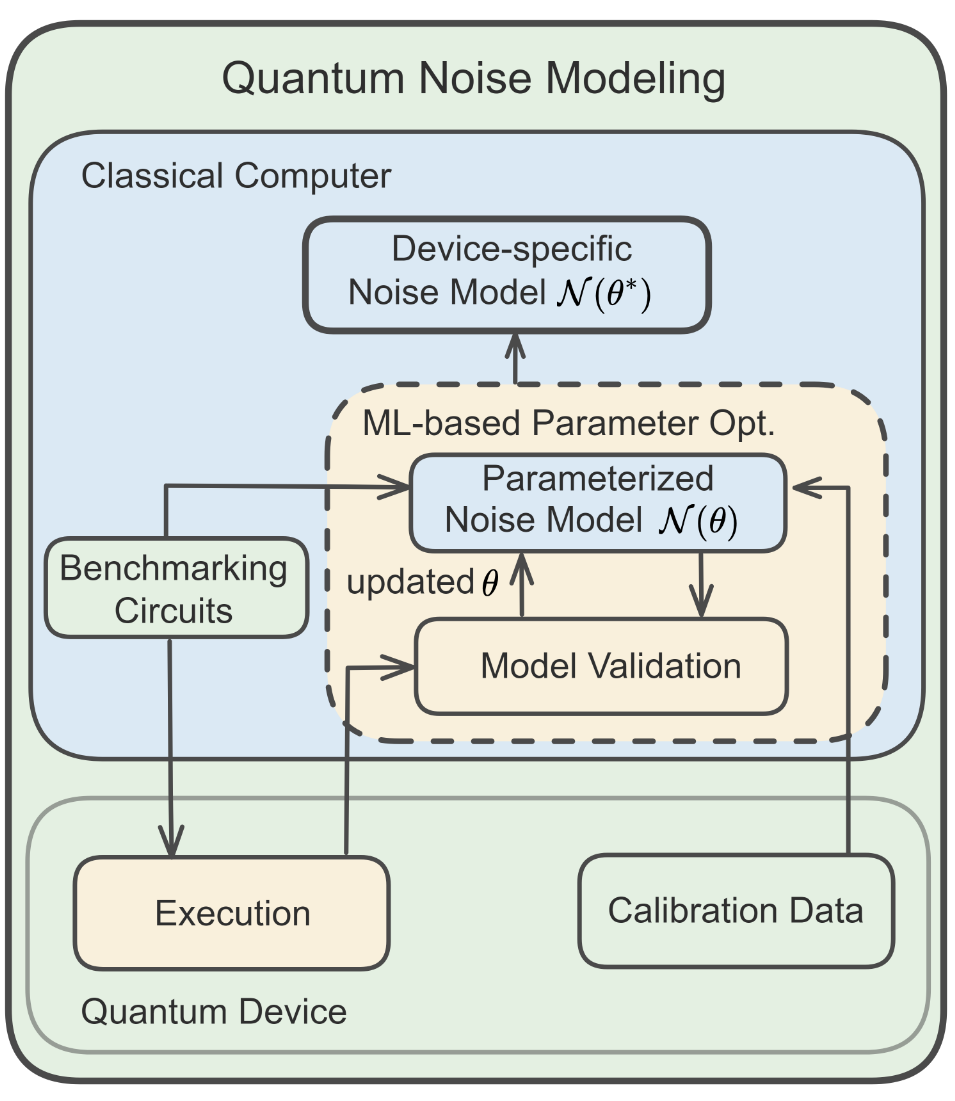
\includegraphics[width=0.5\linewidth]{figures/jie_framework.png}
    \caption{Framework outline for noise modeling in section \ref{sec:jiModeling}}
    \label{fig:ji_framework}
\end{figure}

 % noise parameter modeling
\subsection{System Noise Fingerprinting}
\label{sec:martinaFingerprint}
Martina et al demonstrate that the overall noise fingerprint of a quantum computer can be used to distinguish it from other devices.
The noise fingerprint is a time-ordered sequence of output probabilities at nine points in a specified quantum circuit.
Repeating these circuit measurements either immediately sequential or with delay provides a characterization of how the noise fingerprint of a device evolves over time.
This noise fingerprint is used as the input for a support vector machine (SVM) classifier with the output label of which device was used for the calculation.
Using the trained SVM model, the seven IBM devices used for training could be distinguished with over 99\% accuracy after only three measurements.
This ease of device differentiation based on noise fingerprint indicates that any noise modeling must be both device and time specific - any noise mitigation model for a device must be re-trained several times each day to maintain accuracy.
\cite{martina_learning_2022}
 % device dependence of noise profile
% \subsection{Fidelity Estimation}
\label{sec:vadaliFidelity}

\cite{vadali_quantum_2024}
% approach
\begin{itemize}
    \item Choose existing QC noise model
    \item Generate simple circuits
    \item Model/run noisy circuits
    \begin{itemize}
        \item All gates have same fixed chance of success
        \item Each gate has fixed but different chance of success
        \item Inner gates have reduced chance of success to simulate crosstalk
        \item Full simulation using \verb|cirq| and fidelity distribution for each gate operation
    \end{itemize}
    \item 
\end{itemize}
% results
% improvements/future works
 % circuit fidelity estimation
\subsection{Machine Learning for Quantum Error Mitigation}
\label{sec:liaoMachineMit}

\cite{liao_machine_2024}
% coherent vs incoherent errors
Machine learning can be used to directly mitigate errors as shown bi Liao et al \cite{liao_machine_2024}.
Training data is produced by running the same circuit on both a noisy backend and increasingly complex noise models of real quantum computers as provided by IBM through the \verb|qskit| python package \cite{javadi-abhari_quantum_2024}
Statistical models evaluated are ordinary least squares (OLS), random forest (RF), multi-layer perceptrons (MLP), and graph neural networks (GNN).
Zero noise extrapolation (ZNE) is used as a comparison state-of-the-art noise mitigation reference method.
Of the models evaluated, RF is found to perform the best with a mean error of 0.077 compared to the unmitigated mean error of 0.166 and ZNE with a mean error of 0.118.
A full comparison of tested models can be found in figure \ref{fig:liao_comparison}.

The data generation methods described here - increasingly noisy calculations on a simulated backend - can easily serve as a reference for generating our own training data.  % good here? no need to simulate exact noise sources?
As a key difference, our framework has the additional goal of identifying primary source(s) of noise in the quantum computer and use this information to employ an optimal mitigation method.

\begin{figure}[t]
    \centering
    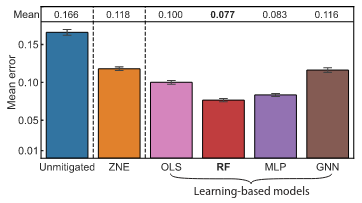
\includegraphics[width=0.5\linewidth]{figures/liao_comparison.png}
    \caption{Comparison of model errors from Liao et al. \cite{liao_machine_2024}}
    \label{fig:liao_comparison}
\end{figure}
 % direct ML mitigation of noise
% \subsection{Deep Learning for Qubit Noise Characterization}
\label{sec:wiseDeepLearn}

\cite{wise_using_2021}


\section{Conclusion}
\label{ch:conclusion}

\bibliographystyle{IEEEtran.bst}
\bibliography{./references.bib}


\end{document}
